%%%%%%%%%%%%%%%%%%%%%%%%%%%%%%%%%%%%%%%%%%%%%%%%%%%%%%%%%%%%
%%  This Beamer template was created by Cameron Bracken.
%%  Anyone can freely use or modify it for any purpose
%%  without attribution.
%%
%%  The current presentation created by Jeferson L. R. Souza (jefecomp) is based on the template created by Cameron Bracken. 
%%  
%%  Small modifications have been introduced and anyone is free to use such modified version.
%%
%% Last Modified: June 14, 2015.

\documentclass[xcolor=x11names,compress]{beamer}

%% General document %%%%%%%%%%%%%%%%%%%%%%%%%%%%%%%%%%
\usepackage{graphicx}
\usepackage{tikz}
\usetikzlibrary{decorations.fractals}
%%%%%%%%%%%%%%%%%%%%%%%%%%%%%%%%%%%%%%%%%%%%%%%%%%%%%%

%Hyperref
\usepackage{hyperref}

%Multirow package
\usepackage{multirow} 

%Math packages
\usepackage{amsmath}
\usepackage{textcomp}


%% Beamer Layout %%%%%%%%%%%%%%%%%%%%%%%%%%%%%%%%%%
\useoutertheme[footline=authorinstitutetitle,subsection=false,shadow]{miniframes}
\useinnertheme{default}
\usefonttheme{professionalfonts}
\usepackage{mathpazo}

\setbeamerfont{title like}{shape=\scshape,series=\bfseries}
\setbeamerfont{frametitle}{shape=\scshape,series=\bfseries}

\setbeamercolor*{lower separation line head}{bg=Green3} 
\setbeamercolor*{upper separation line foot}{bg=Green3} 
\setbeamercolor*{normal text}{fg=black,bg=white} 
\setbeamercolor*{alerted text}{fg=black,bg=black!10} 
\setbeamercolor*{example text}{fg=black} 
\setbeamercolor*{structure}{fg=black}
 
\setbeamercolor*{palette tertiary}{fg=black,bg=black!3} 
\setbeamercolor*{palette quaternary}{fg=black,bg=black!10} 

%%%%%%%%%%%%%%%%%%%%%%%%%%%%%%%%%%%%%%%%%%%%%%%%%%

\setbeamertemplate{blocks}[rounded] [shadow=true]
\setbeamertemplate{frametitle continuation}[from second][(Continuação)]

%%  declaring picture extensions and default path
\DeclareGraphicsExtensions{.png, .jpg, .pdf}
\graphicspath{{pictures/}}

%% Supporting source code lists
\usepackage{listings}
\lstset{breakatwhitespace,
language=Java,
columns=fullflexible,
keepspaces,
breaklines,
tabsize=3, 
showstringspaces=false,
extendedchars=true}

%Text position
\usepackage{textpos}
\setlength{\TPHorizModule}{128mm}
\setlength{\TPVertModule}{96mm}

\usepackage{array}

%Puting text and other float elements over pictures
\usepackage[percent]{overpic}


%% Hyperlinks over all the document
\usepackage{hyperref}

%% Controlling text alignment
\usepackage{ragged2e}

%% Framed text
\usepackage{framed}

%% Math packages
\usepackage{amsmath}

\begin{document}

\title[Qualidade de Software \hskip35mm \insertframenumber / \inserttotalframenumber  \hskip36mm \inserttitlegraphic]{Qualidade de Software \\[4mm]
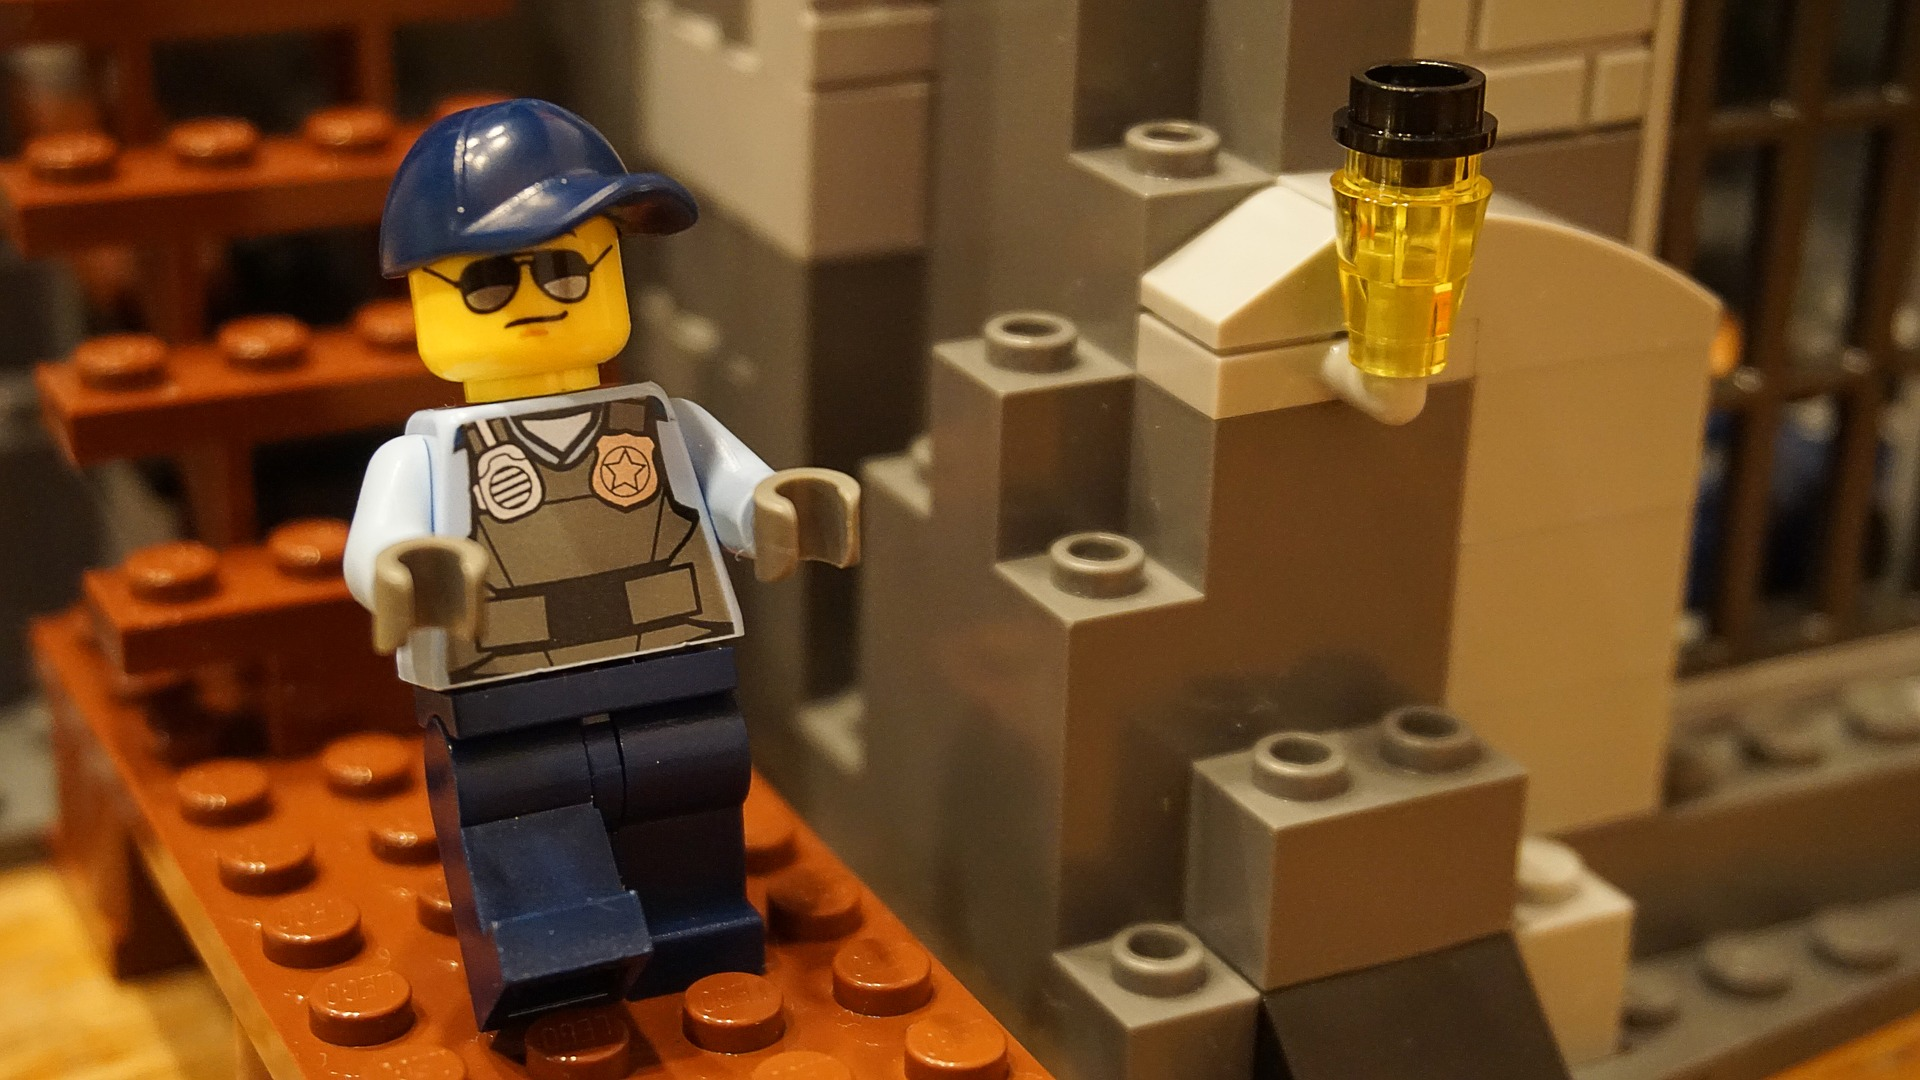
\includegraphics[keepaspectratio,width=.5\textwidth]{lego-ppr}}
\author[@2018 Prof. Jeferson Souza, MSc (jefecomp) - All rights reserved.]{
	\textcolor{blue}{Prof. Jeferson Souza, MSc.} \\[1mm] 
	\textcolor{blue}{\textit{{\footnotesize (jefecomp) }}}\\[1.5mm]
	 \underline{{\footnotesize jeferson.souza@udesc.br}}
	 \vspace*{1mm}
}
\institute[]{
\includegraphics[keepaspectratio,width=.5\textwidth]{template/logo_udesc_joinville_horizontal_assinatura}
}

\date{}

\titlegraphic{
\includegraphics[keepaspectratio,width=.2\textwidth]{template/logo_udesc_joinville_horizontal_assinatura}}

%%%%%%%%%%%%%%%%%%%%%%%%%%%%%%%%%%%%%%%%%%%%%%%%%%%%%%
%%%%%%%%%%%%%%%%%%%%%%%%%%%%%%%%%%%%%%%%%%%%%%%%%%%%%%
\begin{frame}[plain,noframenumbering]
\titlepage
\end{frame}

%%%%%%%%%%%%%%%%%%%%%%%%%%%%%%%%%%%%%%%%%%%%%%%%%%%%%%
%%%%%%%%%%%%%%%%%%%%%%%%%%%%%%%%%%%%%%%%%%%%%%%%%%%%%%
\section{Introdução}
\subsection{Introdução}
\begin{frame}{Qualidade de Software}

\begin{alertblock}{O que é qualidade de software?}
Qualidade de software é uma característica que define (e dá uma indicação) de quão bom um software é. A qualidade de software baseia-se na capacidade de classificar um conjunto de características e comparar essa classificação com uma classificação já pré-estabelecida (ex: ISO 14001).
\end{alertblock}

\end{frame}

\begin{frame}{Etapas da Qualidade}
Existem três importantes etapas relacionadas com a qualidade do software:

\begin{itemize}
\itemsep 5mm

\item Planejamento da qualidade;

\item Garantia da qualidade;

\item Controle da qualidade.

\end{itemize}

\end{frame}

\begin{frame}{Etapas da Qualidade}

\begin{alertblock}{Planejamento da Qualidade}
Visa identificar os padrões de qualidade que devem ser utilizados como base de comparação, e apoio ao desenvolvimento do software.
\end{alertblock}

\end{frame}

\begin{frame}{Etapas da Qualidade}

\begin{alertblock}{Garantia da Qualidade}
Visa assegurar que a qualidade definida nos padrões de qualidade que serão seguidos é atingida, realizando atividades que buscam atestar que os requisitos são atendidos durante o processo de desenvolvimento do software.
\end{alertblock}

\end{frame}

\begin{frame}{Etapas da Qualidade}

\begin{alertblock}{Controle da Qualidade}
Visa realizar atividades que incluem o monitoramento contínuo do processo de desenvolvimento de software, com objetivo de garantir a qualidade do software.  
\end{alertblock}

\end{frame}

\begin{frame}{Objetivos da Qualidade}

\begin{itemize}
\itemsep 5mm

\item Satisfação do cliente;

\item Evitar a ocorrência de erros;

\item Melhoria contínua;

\end{itemize}

\end{frame}

\begin{frame}{Objetivos da Qualidade}

\begin{alertblock}{Satisfação do Cliente}
Todos os requisitos e necessidades do cliente são atingidos, implicando na sua satisfação com o software desenvolvido.
\end{alertblock}

\end{frame}

\begin{frame}{Objetivos da Qualidade}

\begin{alertblock}{Evitar a Ocorrência de Erros}
Evitar (principalmente) que erros ocorram depois da entrega do software ao cliente. A correção de erros tardia é muito mais custosa que a correção do erro ainda em fases iniciais, durante o processo de desenvolvimento.
\end{alertblock}

\end{frame}

\begin{frame}{Objetivos da Qualidade}

\begin{alertblock}{Melhoria Contínua}
Visa garantir que o software desenvolvido, durante a sua evolução e incorporação de novas funcionalidades, continua atingindo os padrões de qualidade exigidos.
\end{alertblock}

\end{frame}

%%%%%%%%%%%%%%%%%%%%%%%%%%%%%%%%%%%%%%%%%%%%%%%%%%%%%%
%%%%%%%%%%%%%%%%%%%%%%%%%%%%%%%%%%%%%%%%%%%%%%%%%%%%%%
\section{Planejamento da Qualidade}
\subsection{Planejamento da Qualidade}

\begin{frame}{Planejamento da Qualidade}

\begin{itemize}
\itemsep 5mm

\item Identifica os padrões de qualidade que serão usados;

\item Determina como os padrões de qualidade poderão ser atingidos pelo software;

\item Pilar da gestão da qualidade.

\end{itemize}

\end{frame}

\begin{frame}{Fases do Planejamento da Qualidade}

\begin{itemize}
\itemsep 5mm

\item Fase inicial - entradas;

\item Ferramentas e técnicas;

\item Fase Final - saídas.

\end{itemize}

\end{frame}

\begin{frame}{Fase Inicial - Entradas}

Na fase inicial devem ser considerados todos os fatores que influenciarão o processo de desenvolvimento do software. Esses fatores são:

\begin{itemize}
\itemsep 5mm

\item Fatores ambientais da empresa;

\item Ativos de processos organizacionais;

\item Declaração do escopo;

\item Plano de gestão do desenvolvimento.

\end{itemize}

\end{frame}

\begin{frame}{Fatores Ambientais da Empresa}

Especifica todos os fatores ambientais da empresa que podem afetar direta, ou indiretamente, o desenvolvimento do software. Esses fatores são:

\begin{itemize}
\itemsep 5mm 

\item Regulamentos;

\item Regras e normas;

\item Diretrizes de agências governamentais.

\end{itemize}

\end{frame}

\begin{frame}{Ativos de Processos Organizacionais}

Envolve o aproveitamento de toda a bagagem histórica da empresa que possa ser útil para o desenvolvimento do software, incluindo:

\begin{itemize}
\itemsep 5mm

\item Políticas, procedimentos, e diretrizes de qualidade;

\item Massa de dados anteriores;

\item Lições aprendidas em desenvolvimentos anteriores.

\end{itemize}

\end{frame}

\begin{frame}{Declaração de Escopo}

Define os limites do desenvolvimento do software, especificando os objetivos do projeto e seus requisitos, bem como as entregas necessárias para atingir os requisitos especificados. Esses limites envolvem:

\begin{itemize}
\itemsep 5mm

\item Custo;

\item Tempo;

\item Recursos utlizados.

\end{itemize}

\end{frame}

\begin{frame}{Plano de Gestão do Desenvolvimento}


\begin{alertblock}{Plano de Gestão do Desenvolvimento}
Inclui as atividades essenciais para definição, coordenação, e integração dos processos de desenvolvimento de software.
\end{alertblock}

\end{frame}

\begin{frame}{Ferramentas e Técnicas}

Engloba os seguintes tópicos:

\begin{itemize}

\itemsep 5mm

\item Análise de custo-benefício;

\item Benchmarking; 

\item Projeto de experimentos;

\item Custo da qualidade;

\item Ferramentas adicionais.
 
\end{itemize}

\end{frame}

\begin{frame}{Análise de Custo-Benefício}

A análise de custo-benefício tem como objetivo equilibrar os custos de gestão da qualidade com os benefícios que essa gestão traz. O principal custo está associado às atividades de gestão da qualidade, enquanto os principais benefícios dessa análise são:

\begin{itemize}

\itemsep 3mm

\item Menor retrabalho;

\item Maior produtividade;

\item Menores custos;

\item Maior satisfação das partes interessadas.

\end{itemize}

\end{frame}

\begin{frame}{Benchmarking}

\begin{alertblock}{Benchmarking}
Envolve a comparação entre práticas de gestão da qualidade que já foram utilizadas em projetos anteriores, a fim de promover idéias de melhoria e medir o desempenho.
\end{alertblock}

\end{frame}

\begin{frame}{Projeto de Experimentos}

\begin{alertblock}{Projeto de Experimentos}
O projeto de experimentos é um método estatístico que auxilia a identificação de fatores que influenciam o processo de desenvolvimento de software. O projeto de experimentos pode ser utilizado, por exemplo, para determinar quais os protocolos de comunicação serão utilizados, de forma que o tempo médio de resposta do produto seja o melhor possível (dentro dos valores esperados).
\end{alertblock}

\end{frame}

\begin{frame}{Custo da Qualidade}

\begin{alertblock}{Custo da Qualidade}
Descreve todos os custos envolvidos no projeto de gestão da qualidade, incluindo  os custos de prevenção de não conformidade com os requisitos, avaliação, e retrabalho. 
\end{alertblock}

\end{frame}

\begin{frame}{Ferramentas Adicionais de Planejamento da Qualidade}

Outras ferramentas são utilizadas para auxiliar todo o planejamento da qualidade de um projeto de software. Essas ferramentas incluem:

\begin{itemize}
\itemsep 3mm

\item Brainstorming;

\item Fluxograma;

\item Matrizes de priorização;

\item Entre outras.

\end{itemize}

\end{frame}

\begin{frame}{Fase Final - Saídas}

Na fase final são produzidos os resultados oriundos de todo o processo de planejamento da qualidade, os quais incluem:

\begin{itemize}
\itemsep 5mm

\item Plano de gestão da qualidade;

\item Métricas de qualidade;

\item Listas de verificação da qualidade;

\item Plano de melhorias no processo;

\item Linha de base da qualidade;

\item Atualizações do plano de gestão do projeto.

\end{itemize}

\end{frame}

\begin{frame}{Plano de Gestão da Qualidade}

\begin{alertblock}{Plano de Gestão da Qualidade}
Descreve como a equipe de gestão do projeto irá implementar as políticas de qualidade dentro do projeto de software. O plano de gestão da qualidade inclui as descrições de ações para controle da qualidade, garantia da qualidade, e melhoria contínua dos processos de desenvolvimento do projeto de software.
\end{alertblock}

\end{frame}

\begin{frame}{Métricas de Qualidade}

\begin{alertblock}{Métricas de Qualidade}
Definem como a qualidade do software desenvolvido será medida. Um exemplo de métrica de qualidade é a cobertura dos testes, a qual especifica um número (porcentagem) que diz quanto do código desenvolvido foi efetivamente testado.
\end{alertblock}

\end{frame}

\begin{frame}{Lista de Verificação da Qualidade}

\begin{alertblock}{Lista de Verificação da Qualidade}
Ferramenta estruturada que especifica uma lista de items, os quais consistem em um conjunto de estapas necessárias ao desenvolvimento, por exemplo, de um componente do software. Cada umas dessas etapas é então verificada para assegurar que as mesmas foram mesmo executadas.
\end{alertblock}

\end{frame}

\begin{frame}{Plano de Melhorias no Processo}

\begin{alertblock}{Plano de Melhorias no Processo}
Permite a identificação de atividades desnecessárias e que não resultam em valor agregado para o software desenvolvido.
\end{alertblock}

\end{frame}

\begin{frame}{Linha de Base da Qualidade}

\begin{alertblock}{Linha de Base da Qualidade}
Registra os objetivos da qualidade do projeto de software, sendo a base para medição e emissão de relatórios do desempenho da gestão e dos processos da qualidade.
\end{alertblock}

\end{frame}

\begin{frame}{Atualizações do Plano de Gestão do Projeto}

\begin{alertblock}{Atualizações do Plano de Gestão do Projeto}
Incorpora ao plano de gestão do projeto o plano de gestão da qualidade e, caso necessário, um plano de melhorias nos processos auxiliares do projeto. Essas incorporações são realizadas através de revisões do plano do projeto, reduzindo o impacto das mudanças (adições, modificações, e exclusões). 

\end{alertblock}

\end{frame}

%%%%%%%%%%%%%%%%%%%%%%%%%%%%%%%%%%%%%%%%%%%%%%%%%%%%%%
%%%%%%%%%%%%%%%%%%%%%%%%%%%%%%%%%%%%%%%%%%%%%%%%%%%%%%
\section{Garantias da Qualidade}
\subsection{Garantias da Qualidade}

\begin{frame}{Garantias da Qualidade}

\begin{alertblock}{Garantias da Qualidade}
A garantia da qualidade visa a execução das atividades de qualidade que foram planejadas, com o objetivo de assegurar que o projeto de software atende os requisitos especificados.
\end{alertblock}

\end{frame}

\begin{frame}{Fases da Garantia da Qualidade}

\begin{itemize}
\itemsep 5mm
\item Fase inicial - entradas;

\item Ferramentas e técnicas;

\item Fase Final - saídas.

\end{itemize}

\end{frame}


\begin{frame}[allowframebreaks]{Fase Inicial - Entradas}

Na fase inicial, a garantia de qualidade toca os seguintes tópicos:

\begin{itemize}
\itemsep 5mm

\item Plano de gestão da qualidade;

\item Métricas de qualidade;

\item Plano de melhorias no processo;

\item Informações sobre o desempenho do trabalho;

\item Solicitações de mudanças aprovadas.

\item Medições de controle da qualidade;

\item Solicitações de mudanças implementadas;

\item Ações corretivas implementadas;

\item Reparo de defeito implementado;

\item Ações preventivas implementadas.

\end{itemize}

\end{frame}

\begin{frame}{Plano de Gestão da Qualidade}

\begin{alertblock}{Plano de Gestão da Qualidade}
Descreve como a garantia da qualidade será realizada dentro do projeto de software.
\end{alertblock}

\end{frame}

\begin{frame}{Métricas da Qualidade e Plano de Melhorias no Processo}

Tanto as métricas da qualidade, quanto o plano de melhorias no processo seguem o que foi definido na etapa de planejamento da qualidade, servindo então como uma das entradas do processo de garantia da qualidade. 

\end{frame}

\begin{frame}{Informações Sobre o Desempenho do Trabalho}

Fornece as seguintes entradas para o processo de garantia da qualidade:

\begin{itemize}
\itemsep 5mm

\item Medidas de desempenho técnico;

\item Situação de entregas do projeto;

\item Ações corretivas necessárias;

\item Relatórios de desempenho.

\end{itemize}

\pause

\begin{alertblock}{\centering \textbf{Utilidade}}
As entradas citadas anteriormente podem ser usadas em áreas como auditorias, revisões de qualidade, e análises de processos.
\end{alertblock}

\end{frame}

\begin{frame}{Solicitações de Mudanças Aprovadas}

As solicitações de mudanças aprovadas podem incluir modificações em:

\begin{itemize}
\itemsep 5mm

\item Métodos de trabalho;

\item Requisitos de produtos;

\item Requisitos de qualidade;

\item Escopo e cronograma.

\end{itemize}

\pause

\begin{alertblock}{\centering \textbf{\textcolor{red}{Importante!}}}
Todas as mudanças devem ser formalmente documentadas por escrito.
\end{alertblock}

\end{frame}

\begin{frame}{Medições de Controle da Qualidade}

\begin{alertblock}{Medições de Controle da Qualidade}
São resultados das atividades de controle da qualidade, os quais fornecem informações importantes na reavaliação, análise dos processos, e padrões de qualidade da organização.
\end{alertblock}

\end{frame}

\begin{frame}{Solicitações de Mudanças Implementadas}

\begin{alertblock}{Solicitações de Mudanças Implementadas}
Descreve as solicitações de mudanças que foram aprovadas e implementadas.
\end{alertblock}

\end{frame}

\begin{frame}{Ações Corretivas Implementadas}

\begin{alertblock}{Ações Corretivas Implementadas}
Descreve as ações corretivas que foram aprovadas e implementadas.
\end{alertblock}

\end{frame}

\begin{frame}{Reparo de Defeito Implementado}

\begin{alertblock}{Reparo de Defeito Implementado}
Descreve as correções de defeitos do produto que foram aprovadas e implementadas.
\end{alertblock}

\end{frame}

\begin{frame}{Ações Preventivas Implementadas}

\begin{alertblock}{Ações Preventivas Implementadas}
Descreve as ações preventivas que foram aprovadas e implementadas.
\end{alertblock}

\end{frame}

\begin{frame}{Ferramentas e Técnicas}

Na etapa da garantia da qualidade, a fase de ferramentas e técnicas envolve os seguintes tópicos:

\begin{itemize}
\itemsep 5mm

\item Ferramentas e técnicas de planejamento da qualidade;

\item Auditorias da qualidade;

\item Análise do processo;

\item Ferramentas e técnicas de controle da qualidade. 

\end{itemize}

\end{frame}

\begin{frame}{Ferramentas e Técnicas de Planejamento da Qualidade}

\begin{alertblock}{Ferramentas e Técnicas de Planejamento da Qualidade}
São as ferramentas e técnicas descritas na etapa de planejamento da qualidade que também podem ser utilizadas para atividades de garantia da qualidade.
\end{alertblock}

\end{frame}

\begin{frame}{Auditorias de Qualidade}

\begin{alertblock}{Auditorias de Qualidade}
Tem o objetivo de identificar políticas, processos, e procedimentos utilizados pelo projeto de software que são ineficientes e com pouca eficácia. 
\end{alertblock}

\end{frame}

\begin{frame}{Análise do Processo}

\begin{alertblock}{Análise do Processo}
Segue o que foi descrito anteriormente no plano de melhorias no processo para identificar as melhorias necessárias, do ponto de vista organizacional e técnico.
\end{alertblock}

\end{frame}

\begin{frame}{Ferramentas e Técnicas de Controle da Qualidade}

\begin{alertblock}{Ferramentas e Técnicas de Controle da Qualidade}
São as ferramentas e técnicas descritas mais a frente, na etapa de controle de qualidade, que também são utilizadas na garantia da qualidade.
\end{alertblock}

\end{frame}

\begin{frame}{Fase Final - Saídas}

Na fase final da garantia da qualidade, as seguintes saídas são esperadas:

\begin{itemize}
\itemsep 5mm

\item Mudanças esperadas;

\item Ações corretivas recomendadas;

\item Atualizações de ativos de processos organizacionais;

\item Atualizações do plano de gestão do projeto.

\end{itemize}

\end{frame}

\begin{frame}{Mudanças Esperadas}

\begin{alertblock}{Mudanças Esperadas}
Engloba a tomada de ações para aumentar a eficácia e eficiência das políticas, processos, e procedimentos da organização.
\end{alertblock}

\end{frame}

\begin{frame}{Ações Corretivas Recomendadas}

\begin{alertblock}{Ações Corretivas Recomendadas}
Engloba a recomendação de ações que podem ser executadas para melhorar a qualidade, e aumentar a eficácia e a eficiência da organização.
\end{alertblock}

\end{frame}

\begin{frame}{Atualizações de Ativos de Processos Organizacionais}

\begin{alertblock}{Atualizações de Ativos de Processos Organizacionais}
Promove atualizações nos padrões de qualidade para fornecer uma garantia que os requisitos são atendidos. Os padrões atualizados são então utilizados na etapa de controle da qualidade.
\end{alertblock}

\end{frame}

\begin{frame}{Atualizações no Plano de Gestão do Projeto}

\begin{alertblock}{Atualizações no Plano de Gestão do Projeto}
As mudanças oriundas da etapa da garantia da qualidade, tais como as atualizações dos padrões de qualidade utilizados, resultam em mudanças no plano de gestão da qualidade, e consequentemente em mudanças no plano de gestão do projeto.
\end{alertblock}

\end{frame}

%%%%%%%%%%%%%%%%%%%%%%%%%%%%%%%%%%%%%%%%%%%%%%%%%%%%%%
%%%%%%%%%%%%%%%%%%%%%%%%%%%%%%%%%%%%%%%%%%%%%%%%%%%%%%
\section{Controle da Qualidade}
\subsection{Controle da Qualidade}

\begin{frame}{Controle da Qualidade}

\begin{alertblock}{Controle da Qualidade}
O controlde da qualidade é parte fundamental para a manutenção da qualidade definida pelo plano de gestão da qualidade. O controle da qualidade envolve o monitoramento de resultados específicos do projeto a fim de verificar se os mesmos atingem os padrões de qualidade exigidos.
\end{alertblock}

\end{frame}

\begin{frame}{Fases do Controle da  Qualidade}

As fases da etapa de controle da qualidade são as seguintes:

\begin{itemize}
\itemsep 5mm

\item Fase inicial - entradas;

\item Ferramentas e técnicas;

\item Fase Final - saídas.

\end{itemize}

\end{frame}

\begin{frame}[allowframebreaks=.7]{Fase Inicial - Entradas}

Na fase inicial do controle da qualidade, os seguintes tópicos são abordados:

\begin{itemize}
\itemsep 5mm

\item Plano de gestão da qualidade;

\item Métricas da qualidade;

\item Listas de verificação da qualidade;

\item Ativos de processos organizacionais;

\item Informações sobre o desempenho do trabalho;

\item Solicitações de mudanças;

\item Entregas.

\end{itemize}

\end{frame}

\begin{frame}{Tópicos do Controle da Qualidade Já Abordados Anteriormente}

Vários tópicos apresentados anteriormente são utilizados como entrada para o processo de controle da qualidade. São eles:

\begin{itemize}
\itemsep 5mm

\item Plano de gestão da qualidade;

\item Métricas da qualidade;

\item Listas de verificação da qualidade;

\item Ativos de processos organizacionais.

\end{itemize}

\end{frame}

\begin{frame}{Informações Sobre o Desempenho do Trabalho}

As informações sobre o desempenho do trabalho realizado no projeto são entradas fundamentais no processo de controle da qualidade. Essas informações incluem:

\begin{itemize}
\itemsep 5mm

\item Medidas de desempenho técnico;

\item Situação atual das entregas do projeto;

\item Implementação das ações corretivas necessárias.

\end{itemize}

\end{frame}

\begin{frame}{Solicitações de Mudanças Aprovadas}

\begin{alertblock}{Solicitações de Mudanças Aprovadas}
As solicitações de mudanças aprovadas podem incluir modificações nos métodos de trabalho e cronograma, cujo a implementação precisa ser verificada.
\end{alertblock}

\end{frame}

\begin{frame}{Entregas}

\begin{alertblock}{Entregas}
Uma entrega é qualquer produto, resultado, ou capacidade para realizar o serviço que precisa ser produzida para terminar o projeto. As entregas são indicadores que são utilizados para medir a eficiência dos processos, e por consequência, a qualidade das atividades desenvolvidas.
\end{alertblock}

\end{frame}

\begin{frame}[allowframebreaks]{Ferramentas e Técnicas}

Na etapa de controle de qualidade várias ferramentas e técnicas são utilizadas para realizar o controle da qualidade. São elas:

\begin{itemize}
\itemsep 5mm

\item Diagrama de causa e efeito;

\item Gráficos de controle;

\item Elaboração de fluxograma;

\item Histograma;

\item Diagrama de pareto;

\item Gráfico de execução;

\item Diagrama de dispersão;

\item Amostragem estatística;

\item Inspeção;

\item Revisão de reparo de defeito.

\end{itemize}

\end{frame}

\begin{frame}[allowframebreaks]{Fase Final - Saídas}

Na fase final do controle da qualidade, os seguintes resultados são esperados:

\begin{itemize}
\itemsep 5mm

\item Medições de controle da qualidade;

\item Reparo do defeito validado;

\item Atualizações da linha de base da qualidade;

\item Ações corretivas recomendadas;

\item Ações preventivas recomendadas;

\item Mudanças solicitadas;

\item Reparo de defeito recomendado;

\item Atualizações de ativos de processos organizacionais;

\item Entregas validadas;

\item Atualizações do plano de gestão do projeto.

\end{itemize}

\end{frame}

\begin{frame}{Medições de Controle da Qualidade}

\begin{alertblock}{Medições de Controle da Qualidade}
As medições de controle da qualidade representam os resultados das atividades que funcionam como indicadores para a gestão da qualidade reavaliar, e analisar os processos e padrões de qualidade da organização.
\end{alertblock}

\end{frame}

\begin{frame}{Reparo de Defeito Validado}

\begin{alertblock} {Reparo de Defeito Validado}
Um defeito representa o não atendimento das especificações ou requisitos de um dado componente. Os reparos de defeito são inspecionados novamente para verificar se serão aceitos ou rejeitados. Os rejeitados podem necessitar de reparo de defeito posterior.
\end{alertblock}

\end{frame}

\begin{frame}{Atualizações da linha de Base da Qualidade}

\begin{alertblock}{Atualizações da Linha de Base da Qualidade}
Especifica as atualizações da linha de base da qualidade que foi apresentada anteriormente.
\end{alertblock}

\end{frame}

\begin{frame}{Ações Corretivas Recomendadas}

\begin{alertblock}{Ações Corretivas Recomendadas}
Envolvem as ações corretivas tomadas como resultado de um indicador do controle da qualidade que diz, que o processo de desenvolvimento excede os parâmetros estabelecidos.
\end{alertblock}

\end{frame}

\begin{frame}{Ações Preventivas Recomendadas}

\begin{alertblock}{Ações Preventivas Recomendadas}
Envolvem ações preventivas tomadas para evitar uma condição que pode exceder os parâmetros estabelecidos em um processo de desenvolvimento.
\end{alertblock}

\end{frame}

\begin{frame}{Mudanças Solicitadas}

\begin{alertblock}{Mudanças Solicitadas}
Derivadas de ações corretivas ou preventivas que exigem uma mudança no projeto. 
\end{alertblock}

\end{frame}

\begin{frame}{Reparo de Defeito Recomendado}

\begin{alertblock}{Reparo de Defeito Recomendado}
A etapa do controle de qualidade pode recomendar o reparo de um defeito identificado.
\end{alertblock}

\end{frame}

\begin{frame}{Atualizações de Ativos de Processos Organizacionais}
As atualizações de ativos de processos organizacionais podem envolver as seguintes ações:

 \begin{itemize}
 \itemsep 5mm
 
\item Registrar o término do uso das listas de verificações;

\item Documentar as lições aprendidas;

\item Validar as entregas realizadas.

\end{itemize}

\end{frame}

\begin{frame}{Atualizações no Plano de Gestão do Projeto}

\begin{alertblock}{Atualizações no Plano de Gestão do Projeto}
Mudanças que resultem do processo de controle da qualidade são refletidas em mudanças no plano de gestão da qualidade, e consequentemente, em mudanças no plano de gestão do projeto.
\end{alertblock}

\end{frame}

%%%%%%%%%%%%%%%%%%%%%%%%%%%%%%%%%%%%%%%%%%%%%%%%%%%%%%
%%%%%%%%%%%%%%%%%%%%%%%%%%%%%%%%%%%%%%%%%%%%%%%%%%%%%%
\section{}

\begin{frame}[plain,allowframebreaks,noframenumbering]{Bibliografia}

\begin{thebibliography}{Pressman, 2001}

\bibitem[Pressman, 2001]{Pressman-2001}

Pressman, R.

\newblock{{\em ``Software Engineering: A Practioner's Approach"}. 4th edition. McGraw-Hill, 2001.}

\bibitem[PMI, 2008]{PMI-2008}

Project Management Institute, Inc.

\newblock{{\em ``A Guide To The Project Management Body Of Knowledge"}. 2008.}

\end{thebibliography}

\end{frame}



\begin{frame}[plain,noframenumbering]

\begin{center}

\includegraphics[keepaspectratio, width=.8\textwidth]{template/happycat-end}
\end{center}
\end{frame}

\end{document}